\section{Xây dựng bộ phân tích ngữ nghĩa}

    Sau khi đã đảm bảo chương trình được xây dựng đúng cú pháp, việc tiếp theo cần làm là cần đảm bảo mỗi câu lệnh trước khi được thực thi xử lý cần đúng ngữ nghĩa. Trong Pandora, việc kiểm tra ngữ nghĩa câu lệnh sẽ được thực hiện trong khi chương trình đang chạy, nên còn được gọi là kiểm tra ngữ nghĩa động (\textbf{dynamic semantic checking}). Bộ phân tích ngữ nghĩa sẽ kiểm tra ngữ nghĩa của mỗi câu lệnh trong chương trình, đảm bảo rằng chúng không chỉ đúng cú pháp mà còn đúng ngữ nghĩa rồi mới được thực thi. Phần lớn các loại lỗi sẽ nằm ở đây, nên việc kiểm tra ngữ nghĩa là một bước quan trọng trong quá trình xây dựng chương trình. Bộ phân tích ngữ nghĩa của ngôn ngữ Pandora bao gồm:

\begin{itemize}
    \item \textbf{Kiểm tra kiểu dữ liệu}: Kiểm tra xem các biến, biểu thức, hàm, \dots có đúng kiểu dữ liệu hay không.
    \item \textbf{Kiểm tra phạm vi}: Kiểm tra xem các biến, hàm, \dots có được sử dụng trong phạm vi đúng hay không.
    \item \textbf{Kiểm tra khởi tạo}: Kiểm tra xem các biến, hàm, \dots có được khởi tạo trước khi sử dụng hay không.
    \item \textbf{Kiểm tra luồng điều khiển}: Kiểm tra các cấu trúc luồng điều khiển (như quay lại, ngắt, tiếp tục) được sử dụng ở các vị trí thích hợp.
    \item \textbf{Kiểm tra lỗi thực thi}: Kiểm tra xem các câu lệnh có thể gây ra lỗi thực thi hay không.
\end{itemize}

\begin{figure}[H]
    \centering
    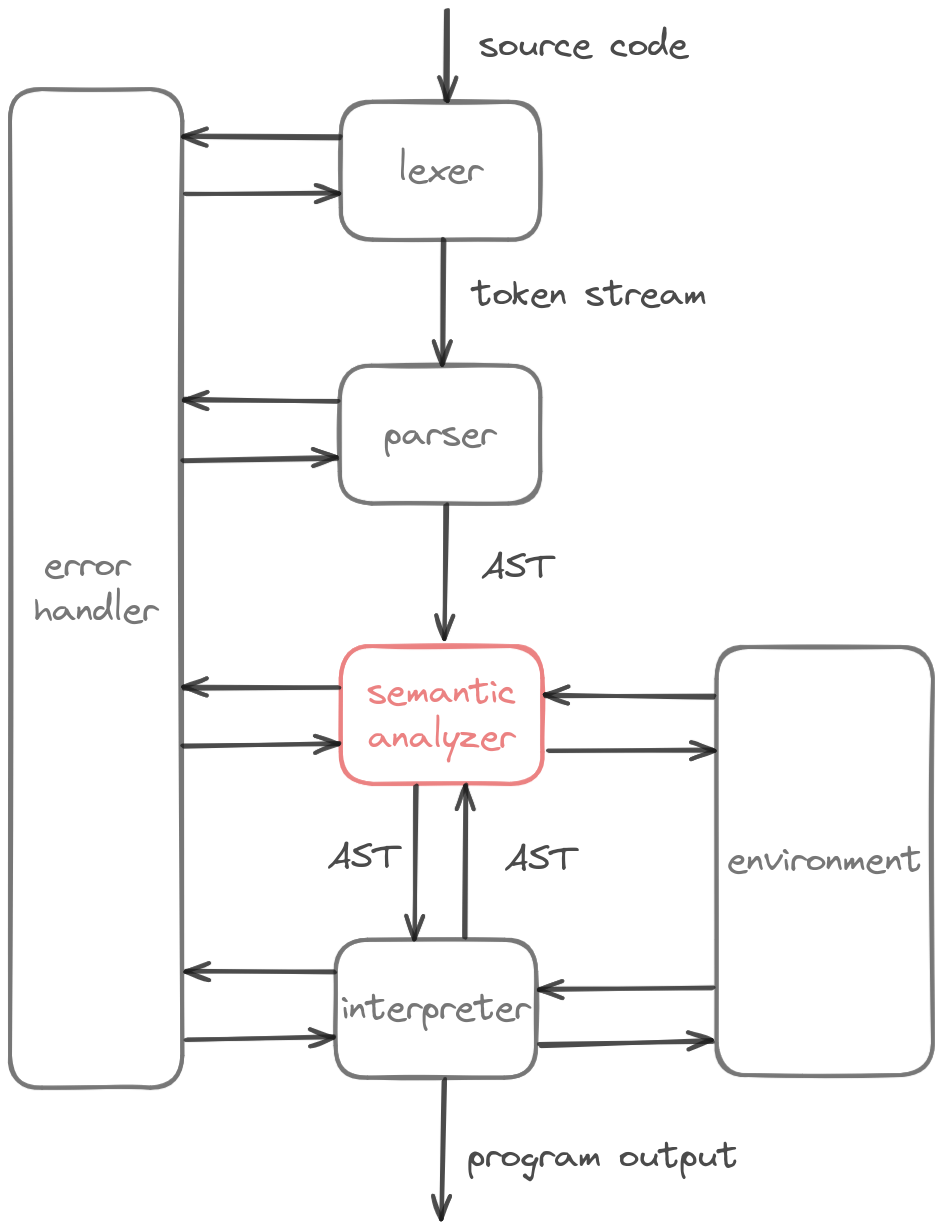
\includegraphics[scale=0.4]{semantic-checking.png}
    \caption{Bộ phân tích ngữ nghĩa trong ngôn ngữ Pandora}
\end{figure}

    Dựa vào sơ đồ trên, ta có thể thấy rằng bộ phân tích ngữ nghĩa sẽ nhận cây cú pháp đã được xây dựng từ bước phân tích cú pháp, sau đó sẽ thực hiện kiểm tra ngữ nghĩa cho từng câu lệnh trong chương trình. Bộ phân tích ngữ nghĩa có thể tương tác với bộ xử lý môi trường để kiểm tra phạm vi, kiểu dữ liệu, \dots của các biến, hàm, \dots trong chương trình. Nếu câu lệnh không đúng ngữ nghĩa, bộ phân tích ngữ nghĩa sẽ thực hiện thông báo lỗi nhờ bộ thông báo lỗi, sau đó chương trình sẽ dừng lại. Nếu câu lệnh đúng ngữ nghĩa, bộ phân tích ngữ nghĩa sẽ chuyển câu lệnh đó cho bộ thông dịch để thực thi. Quá trình kiểm tra ngữ nghĩa sẽ được thực hiện cho đến khi toàn bộ cây cú pháp được kiểm tra xong.

    Ta sẽ phân tích khái quát cách thức hoạt động và xử lý của bộ phân tích ngữ nghĩa trong ngôn ngữ Pandora như sau:

\noindent \textbf{Kiểm tra khai báo (\textit{declaration checking})}

\noindent \textbf{Kiểm tra kiểu dữ liệu (\textit{type checking})}

    Bước này sẽ kiểm tra xem các biến, biểu thức, hàm, \dots có đúng kiểu dữ liệu hay không. Bộ phân tích ngữ nghĩa thường sẽ thực hiện bước này khi thực hiện kiểm tra ngữ nghĩa cho các biểu thức, gán giá trị, truyền tham số, \dots Ví dụ, nếu ta có một biểu thức \kw{a + b}, bộ phân tích ngữ nghĩa sẽ kiểm tra xem biến \kw{a} và \kw{b} có cùng kiểu dữ liệu hay không. Nếu không, bộ phân tích ngữ nghĩa sẽ thông báo lỗi. Phép gán giá trị cũng tương tự, biến và giá trị gán vào biến cần có cùng kiểu dữ liệu. Đối với dữ liệu đặc biệt như mảng, bộ phân tích ngữ nghĩa còn phải thực hiện kiểm tra kích thước mảng (đảm bảo kích thước mảng của biến khi khai báo khớp với số lượng các giá trị có trong mảng), kiểm tra kiểu dữ liệu của mỗi phần tử trong mảng (đảm bảo tất cả các phần tử đều có cùng kiểu dữ liệu), từ đó mới kết luận được kiểu dữ liệu của mảng để quyết định xem có giống với kiểu dữ liệu của biến hay không. Đối với biểu thức gọi hàm, bộ phân tích ngữ nghĩa cần đảm bảo từng tham số truyền vào phải đúng kiểu dữ liệu hàm đó yêu cầu, cũng như kiểu dữ liệu được trả về khi đang thực thi chương trình phải khớp với kiểu dữ liệu trả về hàm yêu cầu. Một số trường hợp khác như biểu thức ép kiểu, bộ phân tích ngữ nghĩa sẽ kiểm tra xem liệu việc chuyển đổi từ kiểu này sang kiểu kia thì có hợp lệ, khả thi không. Ví dụ, việc chuyển từ \kw{3} sang \kw{3.0} (kiểu số nguyên sang kiểu số thực) là hoàn toàn có thể, trong khi việc chuyển từ \kw{2.5} sang \kw{true} (kiểu số thực sang kiểu logic) lại là không hợp lệ trong ngôn ngữ Pandora. Ta cần lưu ý rằng, việc kiểm tra sự khả thi của việc chuyển từ kiểu dữ liệu này sang kiểu dữ liệu khác không có nghĩa là việc ép kiểu đó sẽ luôn hợp lệ. Chẳng hạn, biểu thức ép kiểu \kw{"30" as int} là hợp lệ, tuy nhiên việc cố gắng ép \kw{"hello" as int} lại không hợp lệ, mặc dù đều là biến đổi từ kiểu chuỗi sang kiểu số nguyên. 

    Thông qua việc kiểm tra kiểu dữ liệu, bộ phân tích ngữ nghĩa sẽ đảm bảo kiểu dữ liệu tại mọi thời điểm thực thi của chương trình luôn đúng với những gì ta mong đợi. Từ đó, việc đọc luồng logic cũng như việc phát hiện và sửa lỗi sẽ trở nên dễ dàng hơn.

\noindent Một số ví dụ về việc kiểm tra kiểu dữ liệu
\begin{lstlisting}[]
set a: int = 5; // assign `int` to `int`, correct
set b: float = 5; // assign `int` to `float`, incorrect
set arr: [int; 3] = [1, 2]; // assign `[int; 2]` to `[int; 3]`, incorrect
5 + "5"; // try to add `int` with `str`, not allowed
"hello" as true; // although not correct but still valid in type checking phase
[1, false]; // an array with 2 different types: `int` and `bool`, incorrect
\end{lstlisting}

\noindent \textbf{Kiểm tra phạm vi (\textit{scope checking})}

    Hầu như tất cả các ngôn ngữ lập trình đều phải có phần kiểm tra phạm vi, và Pandora cũng không ngoại lệ. Phạm vi truy cập là một trong những yếu tố quan trọng nhất của ngôn ngữ lập trình. Nó cho ta biết một biến, hàm, \dots nào đó có thể được truy cập và sử dụng hay không. Thông tin về phạm vi truy cập trong ngôn ngữ Pandora sẽ được lưu trữ trong \textbf{môi trường} (một cấu trúc dữ liệu, được phân tích chi tiết ở phần TODO). Bộ phân tích ngữ nghĩa sẽ thông qua dữ liệu có được từ đối tượng môi trường để đánh giá sự hợp lệ trong việc truy cập một biến, hàm, \dots nào đó. Để hiểu hơn về quá trình kiểm tra phạm vi của một biến hay một hàm của bộ phân tích ngữ nghĩa, ta sẽ phân tích ví dụ sau đây:   

\begin{figure}[H]
    \centering
    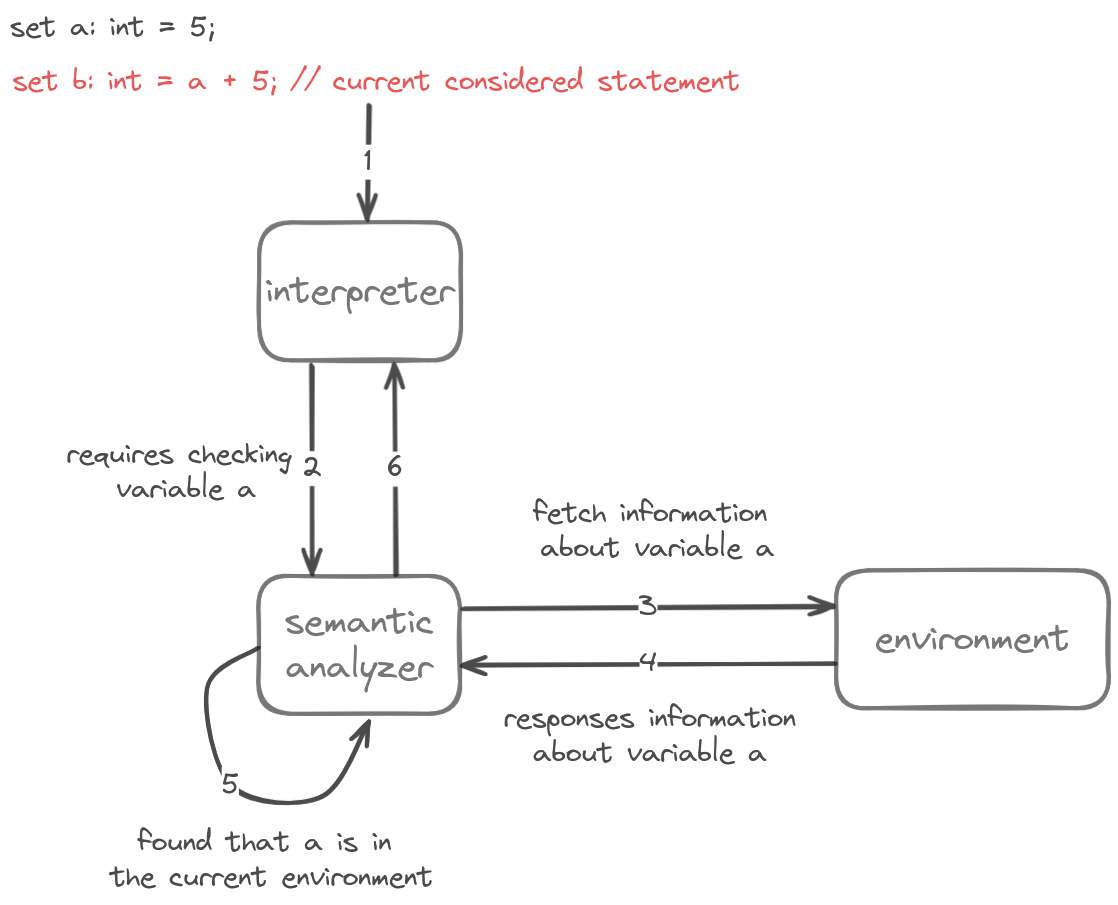
\includegraphics[scale=0.4]{scope-checking.png}
    \caption{Ví dụ về quá trình kiểm tra phạm vi của bộ phân tích ngữ nghĩa}
\end{figure}

    Giả sử câu lệnh đang xét là \kw{set b: int = a + 5}, tức trình thông dịch đã thực thi xong lệnh \kw{set a: int = 5}, và biến \kw{a} đã được lưu vào phạm vi môi trường hiện tại. Khi trình thông dịch đang phân tích tới biến \kw{a} trong biểu thức \kw{a + 5}, nó sẽ yêu cầu bộ phận xử lý ngữ nghĩa kiểm tra phạm vi của biến này. Bộ phân tích ngữ nghĩa sẽ thu thập thông tin của biến \kw{a} trong môi trường hiện tại. Sau khi thấy được thông tin biến \kw{a} có tồn tại trong môi trường. Bộ phân tích ngữ nghĩa sẽ kết thúc quá trình kiểm tra phạm vi của biến \kw{a} và thông báo cho trình thông dịch rằng biến \kw{a} có thể được sử dụng trong biểu thức \kw{a + 5}.

\noindent \textbf{Kiểm tra khởi tạo (\textit{Initialization checking})}

    Trong quá trình thực thi, bộ xử lý ngữ nghĩa sẽ đảm bảo không có trường hợp nào mà biến hoặc hàm được sử dụng mà không được khởi tạo trước đó. Ví dụ, khi truy cập một phần tử trong mảng, hay khi sử dụng một biến, bộ xử lý ngữ nghĩa sẽ kiểm tra xem biến đó đã được khởi tạo hay chưa, nếu chưa, sẽ thông báo lỗi. Bộ xử lý ngữ nghĩa có được thông tin về việc khởi tạo biến từ môi trường, từ đó sẽ kiểm tra xem biến đó đã được khởi tạo hay chưa. Do vậy, bộ xử lý ngữ nghĩa thông thường sẽ thực hiện kiểm tra khởi tạo ngay sau khi kiểm tra phạm vi của biến (bởi cả hai thông tin này đều được lưu trong môi trường) giúp tăng hiệu suất và giảm thời gian thực thi. 

\noindent Ví dụ về việc kiểm tra khởi tạo
\begin{lstlisting}[]
set a: int;
set b: int = a; // a is not initialized
\end{lstlisting}

\noindent \textbf{Kiểm tra luồng điều khiển (\textit{control flow checking})}

    Kiểm tra luồng điều khiển cũng là một bước quan trọng trong quá trình kiểm tra ngữ nghĩa của một chương trình. Bộ phân tích ngữ nghĩa sẽ kiểm tra xem các cấu trúc luồng điều khiển (như quay lại, ngắt, tiếp tục) được sử dụng ở các vị trí thích hợp. Ví dụ, việc sử dụng câu lệnh \kw{br} hoặc câu lệnh \kw{skip} ngoài cấu trúc lặp là không hợp lệ, hay việc sử dụng câu lệnh \kw{yeet} ngoài hàm cũng không hợp lệ.

\noindent Ví dụ về việc kiểm tra luồng điều khiển
\begin{lstlisting}[]
when true {
    br; // not allowed
}
during true {
    skip; // allowed
}
yeet; // not allowed
\end{lstlisting}

\noindent \textbf{Kiểm tra lỗi thực thi (\textit{Running error checking})}

    Trong quá trình thực thi, chẳng hạn khi đang thực thi một biểu thức, mặc dù các biến trong biểu thức được khởi tạo đúng cách, các kiểu dữ liệu khớp nhau, nhưng vẫn có thể xảy ra lỗi thực thi. Ví dụ, khi chia một số cho 0, hoặc khi truy cập một phần tử không tồn tại trong mảng, hoặc khi truy cập một biến không tồn tại, \dots. Bộ phân tích ngữ nghĩa sẽ kiểm tra xem các câu lệnh có thể gây ra lỗi thực thi hay không, và thông báo lỗi nếu cần thiết. 

\noindent Ví dụ về việc kiểm tra lỗi thực thi
\begin{lstlisting}[]
set a: int = 5;
set b: int = 0;
set c: int = a / b; // division by zero
set arr: [int; 3] = [1, 2, 3];
set d: int = arr[3]; // index out of range
\end{lstlisting}

\noindent \textbf{Một số lưu ý về bộ xử lý ngữ nghĩa}

    Việc kiểm tra lỗi thực thi chỉ có thể thực hiện khi chương trình đang thực thi, nên bộ phân tích ngữ nghĩa sẽ không thể kiểm tra hết tất cả các trường hợp có thể xảy ra. Tuy nhiên, việc kiểm tra lỗi thực thi sẽ giúp giảm thiểu việc xảy ra lỗi trong quá trình thực thi chương trình.

\noindent Ví dụ về việc bộ xử lý không phát hiện lỗi
\begin{lstlisting}[]
if true {
    // do something
} alt {
    skip; // not allowed but not detected (because the interpreter will not reach this line)
}

fun test() {
    set b: int = a; // not allowed but not detected (because you are not calling this function)
}
\end{lstlisting}

    Một chương trình đúng ngữ nghĩa không có nghĩa là chương trình không có lỗi. Bộ phân tích ngữ nghĩa chỉ đảm bảo rằng chương trình không có lỗi ngữ nghĩa, nhưng không đảm bảo rằng chương trình sẽ đúng về mặt logic. Do đó, việc kiểm tra ngữ nghĩa chỉ là một phần nhỏ trong quá trình kiểm tra chương trình, và không thể thay thế việc kiểm tra logic của chương trình.

\noindent Ví dụ về việc chương trình đúng ngữ nghĩa nhưng không đúng logic
\begin{lstlisting}[]
fun fib(n: int): int {
    fib(n - 1) + fib(n - 2); // missing base case
}

set a: int = fib(5); // correct in semantic checking phase
\end{lstlisting}

    Trong ví dụ trên, chương trình không có lỗi ngữ nghĩa, nhưng lại không đúng logic. Hàm \kw{fib} sẽ không bao giờ kết thúc vì không có điều kiện dừng, và chương trình sẽ bị lặp vô hạn.

    Sau khi đã xây dựng xong bộ phân tích ngữ nghĩa, ta sẽ tiến hành kết hợp bộ phân tích ngữ nghĩa với bộ thông dịch để thực thi chương trình. Quá trình này sẽ được thực hiện trong bước thực thi chương trình.
